\documentclass[10pt,a4paper]{article}
\usepackage[utf8]{inputenc}
\usepackage{amsmath}
\usepackage{amsfonts}
\usepackage{amssymb}
\usepackage{makeidx}
\usepackage{graphicx}
\usepackage{parskip}
\usepackage[left=2cm,right=2cm,top=2cm,bottom=2cm]{geometry}
\author{Miguel Angel Xamie Diaz Fuentes/Jimenez Cortes Raul}

\begin{document}
\begin{center}
\begin{LARGE}
\textbf{INGENIERÍA MECATRÓNICA}\\
\end{LARGE}
{\large Sistemas Electrónicos De Interfaz}\\
\begin{figure}[hbtp]
\centering

\includegraphics[scale=0.80]{UPZMG_Mecatr_nica.png}
\end{figure} 
\begin{center}
\begin{LARGE}
EV-1-3-Circuitos De Control De Voltaje Y Corriente Con Transistores.
\end{LARGE}
\end{center}

\begin{Large}
\textbf{Alumnos}
\\\textit{Miguel Ángel Xamie Diaz Fuentes\\Raul Jimenez Cortez}
\textbf{\\Maestro}
\\\textit{Morán Garabito Carlos Enrique}
\textbf{\\Fecha de Entrega}
\\\textit{01/11/2019}
\textbf{\\Grupo}
\\\textit{4-B}
\end{Large}

\end{center}

\footnote{Universidad Politécnica De La Zona Metropolitana De Guadalajara} 

\newpage

\section{Objetivo}
En esta practica se obtendrá como resultado lograr encender un foco de 127 V con un potenciómetro el cual fomente tres tipos de intensidad bajo, intermedio y alto.

\section{Materiales}

\begin{itemize}

\item Resistencia 10k.
\item Potenciómetro 500k.
\item Fuentes de Poder.
\item Multímetro.
\item Foco.
\item Cables Duponk.
\item Protoboards.
\item Clavija 127V.
\item Triac y Diack.

\end{itemize}

\section{Marco Teórico}

Un regulador de tensión o regulador de voltaje es un dispositivo electrónico diseñado para mantener un nivel de tensión constante.
Los reguladores electrónicos de tensión se encuentran en dispositivos como las fuentes de alimentación de los computadores, donde estabilizan las tensiones de Corriente Continua usadas por el procesador y otros elementos. En los alternadores de los automóviles y en las plantas generadoras, los reguladores de tensión controlan la salida de la planta. En un sistema de distribución de energía eléctrica, los reguladores de tensión pueden instalarse en una subastación o junto con las líneas de distribución de forma que todos los consumidores reciban una tensión constante independientemente de cuanta potencia exista en la línea.\\

\textbf{Reguladores integrados}
Hoy en día es más común encontrar en las fuentes de alimentación reguladores integrados, normalmente son componentes muy parecidos a los transistores de potencia, suelen tener tres terminales, uno de entrada, un común o masa, y uno de salida, tienen una capacidad de reducción del rizado muy alta y normalmente solo hay que conectarles un par de condensadores. Existen circuitos reguladores con un gran abanico de tensiones y corrientes de funcionamiento. La serie más conocida de reguladores integrados es la 78xx y la serie 79xx para tensiones negativas. Los de mayor potencia necesitarán un disipador de calor, este es el principal problema de los reguladores serie lineales tanto discretos como integrados, al estar en serie con la carga las caídas de tensión en sus componentes provocan grandes disipaciones de potencia. Normalmente estos reguladores no son buenos para aplicaciones de audio por el ruido que pueden introducir en pre-amplificadores. Para ello es mejor utilizar regulación con componentes discretos o reguladores tipo LDO de bajo ruido. \\

\textbf{Reguladores conmutados:}
Los reguladores conmutados solucionan los problemas de los dispositivos anteriormente citados, poseen mayor rendimiento de conversión, ya que los transistores funcionan en conmutación, reduciendo así la potencia disipada en estos y el tamaño de los disipadores. Se pueden encontrar este tipo de fuentes en los ordenadores personales, en electrodomésticos, reproductores DVD, etc, una desventaja es la producción de ruido electromagnético generado por la conmutación a frecuencias elevadas, teniendo que apantallar y diseñar correctamente la PCB (Placa de Circuito Impreso) del convertidor.\\

\footnote{Universidad Politécnica De La Zona Metropolitana De Guadalajara}
\newpage

\textbf{Reguladores electromecánicos:}
Los reguladores electromecánicos basan su principio de funcionamiento en un auto transformador de columna, sobre la cual se dispone un cursor accionado por un servomotor, que en su recorrido suma o resta espiras. Este movimiento de auto ajuste es controlado por un comando electrónico, que se activa cada vez que la tensión de salida se desvía de su valor de calibración, ajustándose automáticamente y con ello mantiene permanentemente la tensión de salida estable, la respuesta es lenta a las variaciones rápidas de tensión. Las ventajas que ofrece este principio son que cuenta con una alta precisión 1,5 por ciento.

\section{Desarrollo}
\textbf{Etapa 1}

Primero se realizo el circuito de acuerdo al diagrama dado por el profesor en clase un día antes de la practica para realizarla en físico. En la primera parte de esta practica era utilizar el circuito de PLC por las 3 interfaces de entrada, control y salida poder controlar el voltaje y la corriente a través de los relevadores. A continuacion se muestra el circuito de PLC.

\begin{figure}[hbtp]
\centering
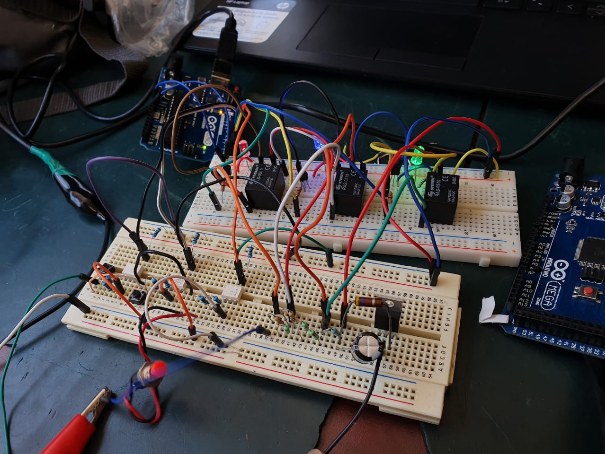
\includegraphics[scale=0.60]{1.png}
\end{figure}

\textbf{Etapa 2}

En esta etapa era poner las etapas de nivel de intensidad del foco incrementando las resistencias y poner las salida de esos niveles a los relevadores para que la corriente a la hora de activar cada nivel fluya por donde halla menos resistencia.

Eso se parte del circuito se puede observar en la esquina inferior derecha o a continuación en la imagen.

\begin{figure}[hbtp]
\centering
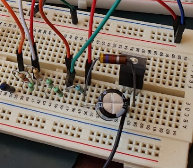
\includegraphics[scale=0.60]{2.png}
\end{figure}
 

\footnote{Universidad Politécnica De La Zona Metropolitana De Guadalajara}
\newpage

El circuito así tal cual esta armado no funciono y nos hizo retrasar la practica por mas tiempo hasta que tuviéramos el diagrama correcto que utilizaríamos para que el foco pudiera disminuir el voltaje y la corriente de manera correcta y de acuerdo a como se pide la practica. Las modificaciones tienen como diferencia agregar un potenciómetro, un diac, un capacitor de diferente valor y una resistencia de 10k hacia la entrada del potenciómetro.

\textbf{Etapa 3}

Para armarlo fue muy rápido, no tuvimos algún problema grande que no dejara realizar la practica a tiempo ya sea un corto o material equivocado excepto por la resistencia que iba al potenciómetro. Se solicitaba una de 1k pero esta al disminuir la resistencia del potenciómetro aria que se quemara, así que se cambio por una de 10k.

El diagrama del circuito nuevo es el siguiente:


\begin{figure}[hbtp]
\centering
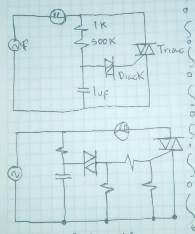
\includegraphics[scale=0.80]{3.png}
\end{figure}

\textbf{Etapa 4}

Se realizo el conjunto de estos dos sistemas y se observo que efectivamente se regulaba la corriente y el voltaje con este sistema de control, no tenemos fotografías ya que no teníamos el teléfono en disposición. Pero el profesor observo el funcionamiento y control del mismo.

A continuación se muestra un diagrama del PLC.


\begin{figure}[hbtp]
\centering
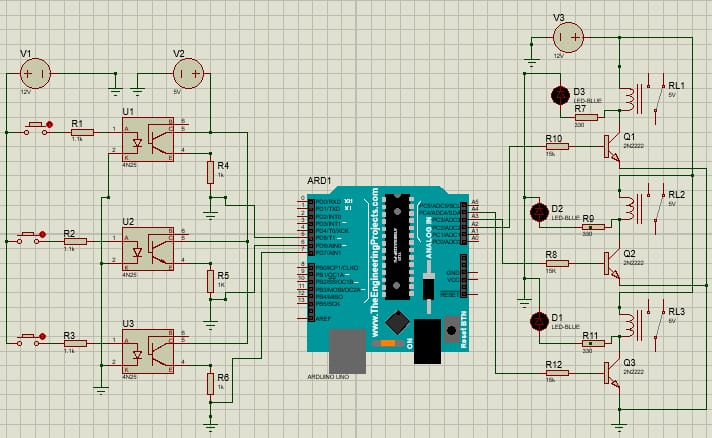
\includegraphics[scale=0.60]{Diagrama.png}
\end{figure}

\footnote{Universidad Politécnica De La Zona Metropolitana De Guadalajara}

Como se puede observa del lado izquierdo las terminales común y abierto se utilizaran como control para que la corriente fluyera a la hora de activar la compuerta eligiendo el nivel de intensidad. La conexión se puede ver en la imagen de la etapa 2.

\section{Cálculos}

Para el uso de las resistencias correctas se realizaron cálculos de acuerdo al modelo del optoacomplador y una que esta en función de salida hacia el arduino y la recibe el transistor (2N2222).\\
Datos:\\

Voltajes de entrada: 12v, 5v.\\

Datos del optoacoplador:\\

If = 10mA ------
Vf = 1.12v\\

{\Large $ R_{Led} = {\Large \frac{(12v - 1.15v)}{10mA}}$} \\

Aquí se toman los parámetros del optoacoplador (425).\\

{\Large $R_{Led} = 1.085\Omega$}\\

{\Large $R_{Transistor} = \frac{(5v - 0.6v)*250}{12mA}$}\\

Aquí se toman los parámetros del relevador y de la medida del transistor con el multimetro.\\

{\Large $R_{Transistor} = 1.528K\Omega$}\\

Por ultimo también determinamos la potencia.\\

$ W = I^2 R $\\ 

$ W = (10mA)(1.100\Omega)$\\

$ W = 0.11w $\\

\textbf{Corriente de los niveles del foco:}

$ I_{Nivel Bajo} = \frac{120v}{420k} = 0.25A $

$ I_{Nivel Medio} = \frac{80v}{280k} = 0.28A $

$ I_{Nivel Alto} = \frac{60v}{120k} = 0.5A $

$ I_{Nivel Bajo} = 0.25 * 480 = 120v $

$ V_{Nivel Medio} = 0.28A * 280k = 78.4v $

$ V_{Nivel Alto} = 0.5A * 120k = 60v $


\footnote{Universidad Politécnica De La Zona Metropolitana De Guadalajara}


\section{Conclusiones}

La competencia aprendida en esta practica fue muy didáctica se alargo un poco el plazo de entrega pero se pudo realizar adecuadamente realizando modificaciones en la etapa final del circuito. Debemos tomar en cuenta que el circuito se divide en 3 etapas, tenemos la primera que son las entradas, la segunda que es el control y la tercera que son las salidas, en la salidas se utilizan los relevadores para dividir la corriente que va hacia el foco. Tenemos niveles de intensidad, la primera es (420k ohms) que es el nivel de baja intensidad, la segunda es (280k ohms) nivel de media intensidad y por ultimo (120k ohms).\\

La modificación que se hizo fue agregar un DIAC, un potenciómetro de 500k y un capacitor de 1uF. La instalación fue fácil y no tuvimos algún problema. Se pudo comprender el control de voltaje y corriente a través de las etapas de control.

\bibliography{Referencia}
\begin{thebibliography}{X}
\bibitem{Baz} Pansini, Anthony J. (2007). Electrical Distribution Engineering (en inglés). The Fairmont Press. Consultado el 15 de septiembre de 2012..


\bibitem{Baz}  Microelectronics Failure Analysis (en inglés). ASM International. 2004. ISBN 0-87170-804-3. Consultado el 15 de septiembre de 2012.
\end{thebibliography}

\bibliographystyle{plain}
\footnote{Universidad Politécnica De La Zona Metropolitana De Guadalajara}
\end{document}